% Created 2021-09-01 Wed 09:50
% Intended LaTeX compiler: pdflatex
\documentclass{article}
\usepackage[utf8]{inputenc}
\usepackage[T1]{fontenc}
\usepackage{graphicx}
\usepackage{grffile}
\usepackage{longtable}
\usepackage{wrapfig}
\usepackage{rotating}
\usepackage[normalem]{ulem}
\usepackage{amsmath}
\usepackage{textcomp}
\usepackage{amssymb}
\usepackage{capt-of}
\usepackage{hyperref}

\usepackage[a4paper,left=0.5in,right=0.5in,top=0.5in,bottom=1in]{geometry}
\usepackage{float}
\DeclareUnicodeCharacter{2212}{-}
\setcounter{secnumdepth}{0}
\author{Tzong Lin Chua}
\date{\today}
\title{EE4C10 Analog Circuit Design Fundamentals\\\medskip
\large Homework Assignment I }
\hypersetup{
 pdfauthor={Tzong Lin Chua},
 pdftitle={EE4C10 Analog Circuit Design Fundamentals},
 pdfkeywords={},
 pdfsubject={},
 pdfcreator={Emacs 27.1 (Org mode 9.5)}, 
 pdflang={English}}
\begin{document}

\maketitle
\tableofcontents


\section{Problem 1}
\label{sec:org9affcb2}
For \(I_{D} = 40 \mu{}A\):
\begin{equation*}
\begin{aligned}
I_{D} &= \frac{1.8V - V_{D}}{R} \\
V_{D} &= 1.8V - I_{D}R \\
\underline{V_{D} &= 1.0V}
\end{aligned}
\end{equation*}
Saturation region:
\begin{equation*}
\begin{aligned}
V_{GS} &= 1.0V > V_{TH} \\
V_{GS} - V_{TH}&= 0.4V < V_{DS} \\
\end{aligned}
\end{equation*}

\begin{enumerate}
\item \(\lambda = 0 V^{-1}\)
\begin{equation*}
\begin{aligned}
I_{D} &= \frac{\mu_{n}C_{OX}}{2}\frac{W}{L}(V_{GS} - V_{TH})^{2} \\
L &= \frac{\mu_{n}C_{OX}}{2}\frac{W}{I_{D}}(V_{GS} - V_{TH})^{2} \\
\underline{L &= 0.39 \mu{}m}
\end{aligned}
\end{equation*}

\item \(\lambda = 0.06 V^{-1}\)
\begin{equation*}
\begin{aligned}
I_{D} &= \frac{\mu_{n}C_{OX}}{2}\frac{W}{L}(V_{GS} - V_{TH})^{2}(1 + \lambda{}V_{DS}) \\
L &= \frac{\mu_{n}C_{OX}}{2}\frac{W}{I_{D}}(V_{GS} - V_{TH})^{2}(1 + \lambda{}V_{DS}) \\
\underline{L &= 0.41 \mu{}m}
\end{aligned}
\end{equation*}
\end{enumerate}

\section{Problem 2}
\label{sec:org3732bc0}
\begin{enumerate}
\item Bulk of the transistors are connected to the source, \(V_{B} = V_{S}\)
\begin{equation*}
\begin{aligned}
V_{TH} &= V_{TH0} + \gamma{}(\sqrt{2\varphi_{F} + V_{BS}} - \sqrt{|2\varphi_{F}|}) \\
V_{TH} &= V_{TH0} = 0.33 V \\
\end{aligned}
\end{equation*}
\begin{enumerate}
\item Transistor M\textsubscript{1}
\begin{equation*}
\begin{aligned}
V_{SG} &= 2.5V - 1.7 V  = 0.8 V \\
\\
I_{D} &= \frac{\mu_{p}C_{OX}}{2}\frac{W}{L}(V_{SG} - V_{TH})^{2} \\
W &= \frac{2LI_{D}}{\mu_{p}C_{OX}}\frac{1}{(V_{SG} - V_{TH})^{2}} \\
W_{1} &= 2.72 \mu{}m
\end{aligned}
\end{equation*}

\item Transistor M\textsubscript{2}
\begin{equation*}
\begin{aligned}
V_{SG} &= 1.7 V - 1 V  = 0.7 V \\
\\
W &= \frac{2LI_{D}}{\mu_{p}C_{OX}}\frac{1}{(V_{SG} - V_{TH})^{2}} \\
W_{2} &= 4.38 \mu{}m
\end{aligned}
\end{equation*}

\item Transistor M\textsubscript{3}
\begin{equation*}
\begin{aligned}
V_{SG} &= 1 V \\
\\
W &= \frac{2LI_{D}}{\mu_{p}C_{OX}}\frac{1}{(V_{SG} - V_{TH})^{2}} \\
W_{3} &= 1.37 \mu{}m
\end{aligned}
\end{equation*}
\end{enumerate}

\item Bulk terminals are attached to the V\textsubscript{DD}, \(V_{B} = V_{DD}\).
\begin{enumerate}
\item Transistor M\textsubscript{1}
\begin{equation*}
\begin{aligned}
V_{BS} &= 2.5 V - 2.5 V = 0 V \\
\\
V_{TH} &= V_{TH0} + \gamma{}(\sqrt{2\varphi_{F} + V_{BS}} - \sqrt{|2\varphi_{F}|}) \\
V_{TH} &= V_{TH0} = 0.33 V \\
\\
W &= \frac{2LI_{D}}{\mu_{p}C_{OX}}\frac{1}{(V_{SG} - V_{TH})^{2}} \\
W_{1} &= 2.72 \mu{}m
\end{aligned}
\end{equation*}

\item Transistor M\textsubscript{2}
\begin{equation*}
\begin{aligned}
V_{BS} &= 2.5 V - 1.7 V = 0.8 V \\
\\
V_{TH} &= V_{TH0} + \gamma{}(\sqrt{2\varphi_{F} + V_{BS}} - \sqrt{|2\varphi_{F}|}) \\
V_{TH} &= V_{TH0} = 0.43 V \\
\\
W &= \frac{2LI_{D}}{\mu_{p}C_{OX}}\frac{1}{(V_{SG} - V_{TH})^{2}} \\
W_{2} &= 8.23 \mu{}m
\end{aligned}
\end{equation*}

\item Transistor M\textsubscript{3}
\begin{equation*}
\begin{aligned}
V_{BS} &= 2.5 V - 1.0 V = 1.5 V \\
\\
V_{TH} &= V_{TH0} + \gamma{}(\sqrt{2\varphi_{F} + V_{BS}} - \sqrt{|2\varphi_{F}|}) \\
V_{TH} &= V_{TH0} = 0.49 V \\
\\
W &= \frac{2LI_{D}}{\mu_{p}C_{OX}}\frac{1}{(V_{SG} - V_{TH})^{2}} \\
W_{3} &= 2.31 \mu{}m
\end{aligned}
\end{equation*}
\end{enumerate}
\end{enumerate}

\section{Problem 3}
\label{sec:org4723046}
\begin{enumerate}
\item Testbench and I\textsubscript{D}-V\textsubscript{GS} characteristics of NMOS and PMOS
\begin{enumerate}
\item NMOS
\begin{enumerate}
\item Testbench
\begin{figure}[H]
\centering
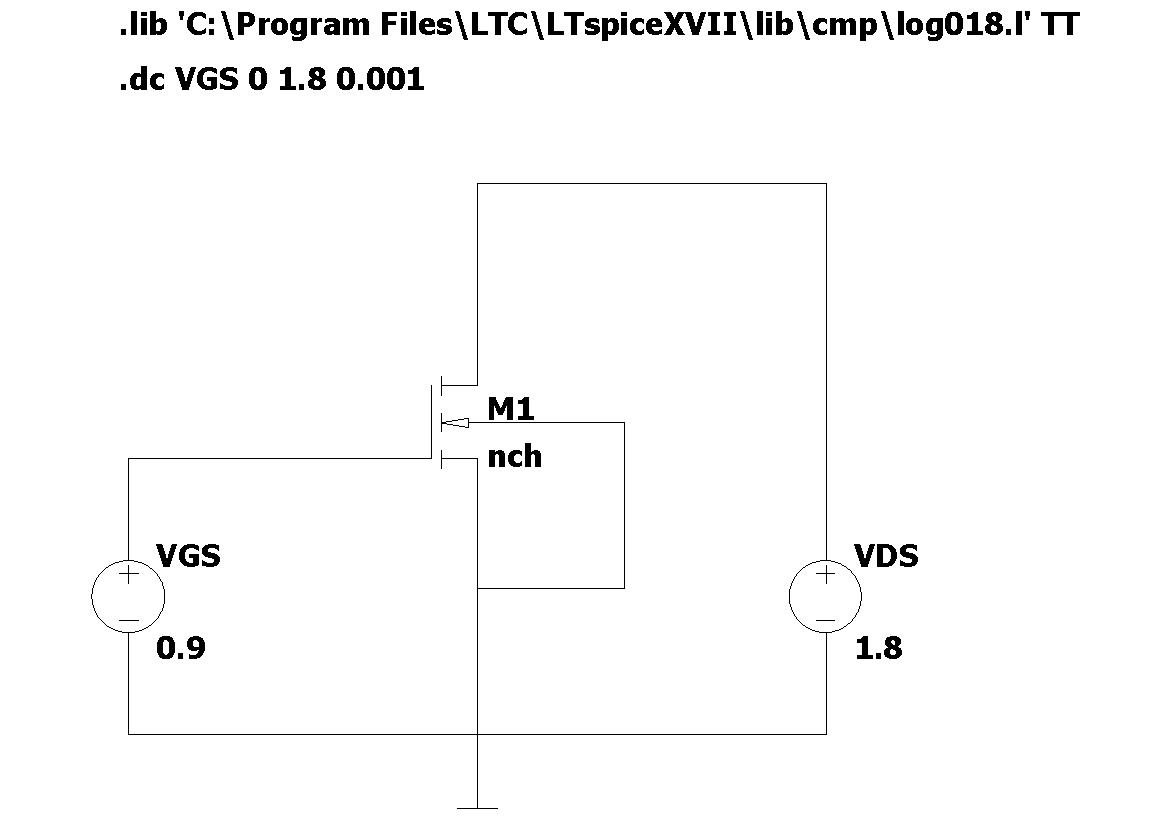
\includegraphics[width=300px]{img/q3/a/nmos-testbench.pdf}
\caption{\label{fig:nmos-testbench}NMOS Testbench}
\end{figure}
\item I\textsubscript{D}-V\textsubscript{GS}
\begin{figure}[H]
\centering
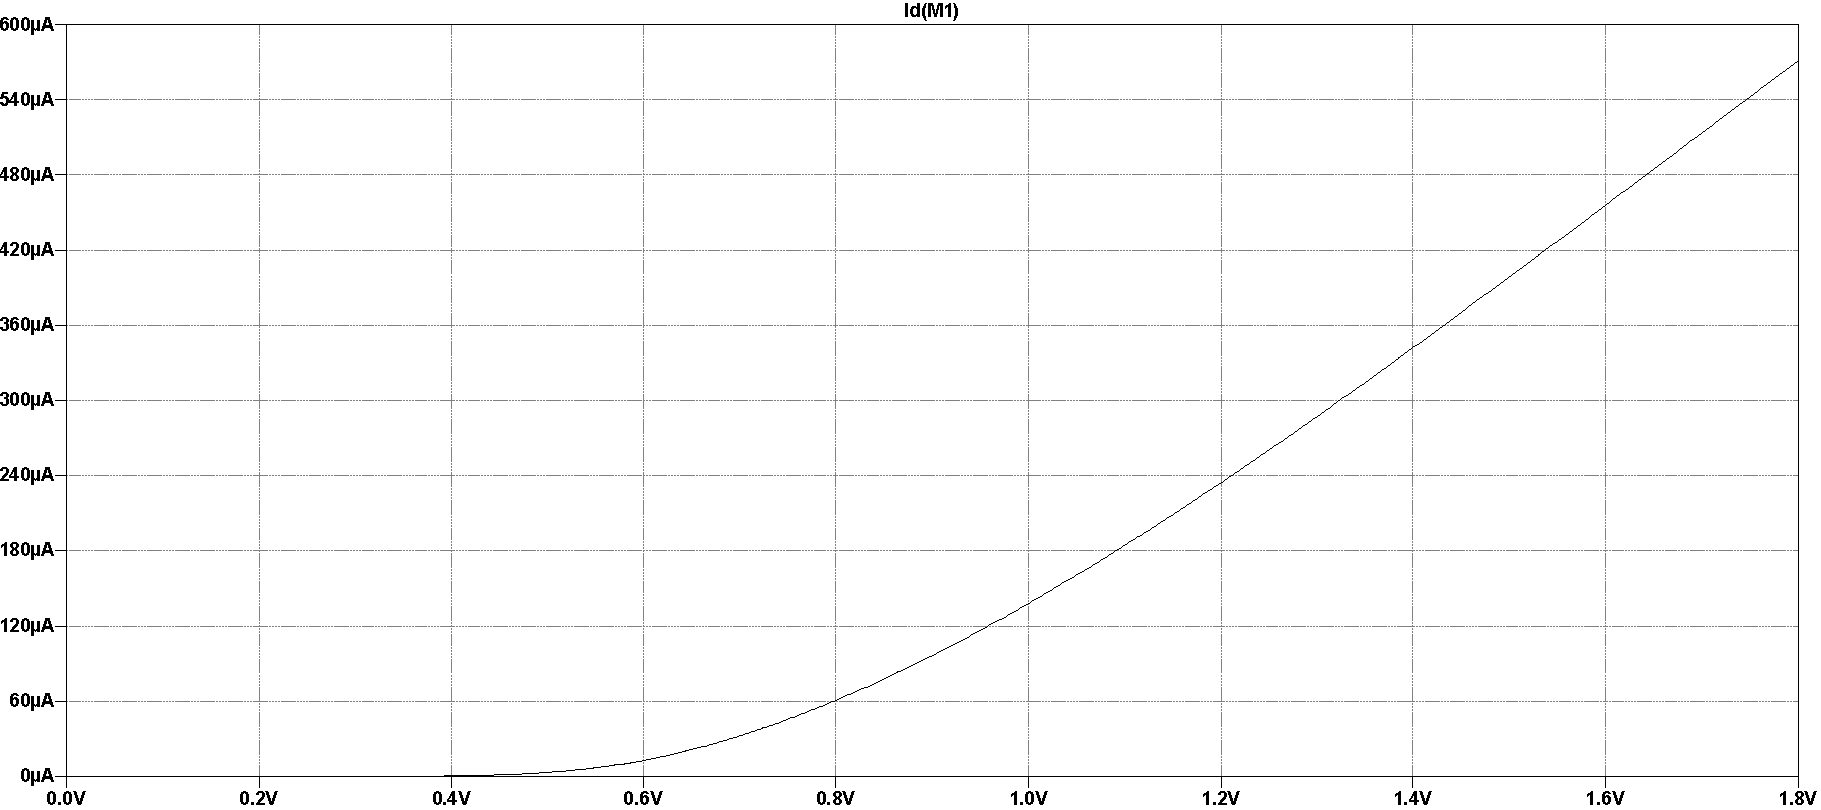
\includegraphics[width=.9\linewidth]{img/q3/a/nmos-id-vgs.pdf}
\caption{\label{fig:nmos-id-vgs}NMOS I\textsubscript{D}-V\textsubscript{GS}}
\end{figure}
\end{enumerate}
\item PMOS
\begin{enumerate}
\item Testbench
\item I\textsubscript{D}-V\textsubscript{GS}
\end{enumerate}
\end{enumerate}
\item \(\mu_{n(p)}C_{OX}\) and \(V_{THn(p)}\)

Assuming that channel length modulation is negligible, \(V_{THn}\) for NMOS can be derived
from the following relation:
\begin{equation}
\begin{aligned}
I_{D} &= \frac{\mu_{n}C_{ox}}{2} \frac{W}{L} (V_{GS} - V_{THn})^2 \\
\frac{2 I_{D}}{\mu_{n}C_{ox}}\frac{L}{W} &=  (V_{GS} - V_{THn})^2 \\
\sqrt{\frac{2 I_{D}}{\mu_{n}C_{ox}}\frac{L}{W}} &=  V_{GS} - V_{THn} \\
\end{aligned}
\end{equation}
V\textsubscript{THn} is the x-axis intercept when the saturation region is extrapolated.
In the case of PMOS, the relation becomes:
\begin{equation}
\begin{aligned}
\sqrt{\frac{2 I_{S}}{\mu_{p}C_{ox}}\frac{L}{W}} &=  V_{SG} - V_{THp} \\
\end{aligned}
\end{equation}
For deriving \(\mu_{n}C_{OX}\), since V\textsubscript{THn(p)} is constant at specific temperatures.
Differentiating both sides with respect to V\textsubscript{GS(SG)} will give:
\begin{equation*}
\begin{aligned}
\frac{d}{dV_{GS}}\sqrt{\frac{2 I_{D}}{\mu_{n}C_{ox}}\frac{L}{W}} &=  \frac{d}{dV_{GS}}(V_{GS} - V_{THn}) \\
\frac{1}{2} \frac{dI_{D}}{dV_{GS}} \sqrt{\frac{2}{I_{D}\mu_{n}C_{ox}}\frac{L}{W}} &=  1 \\
\sqrt{\mu_{n}C_{ox}} &= \frac{1}{2} \frac{dI_{D}}{dV_{GS}} \sqrt{\frac{2}{I_{D}}\frac{L}{W}} \\
\mu_{n}C_{ox} &= \frac{1}{2} \frac{L}{W} \frac{1}{I_{D}}(\frac{dI_{D}}{dV_{GS}})^{2} \\
\mu_{n}C_{ox} &= \frac{1}{6 I_{D}}(\frac{dI_{D}}{dV_{GS}})^{2} \\
\end{aligned}
\end{equation*}
In the case for PMOS, the relation becomes:
\begin{equation*}
\begin{aligned}
\mu_{p}C_{ox} &= \frac{1}{6 I_{S}}(\frac{dI_{S}}{dV_{SG}})^{2} \\
\end{aligned}
\end{equation*}

\begin{enumerate}
\item NMOS
\begin{enumerate}
\item \(\mu_{n}C_{OX} = 306 \mu{}AV^{-2}\)
\begin{figure}[H]
\centering
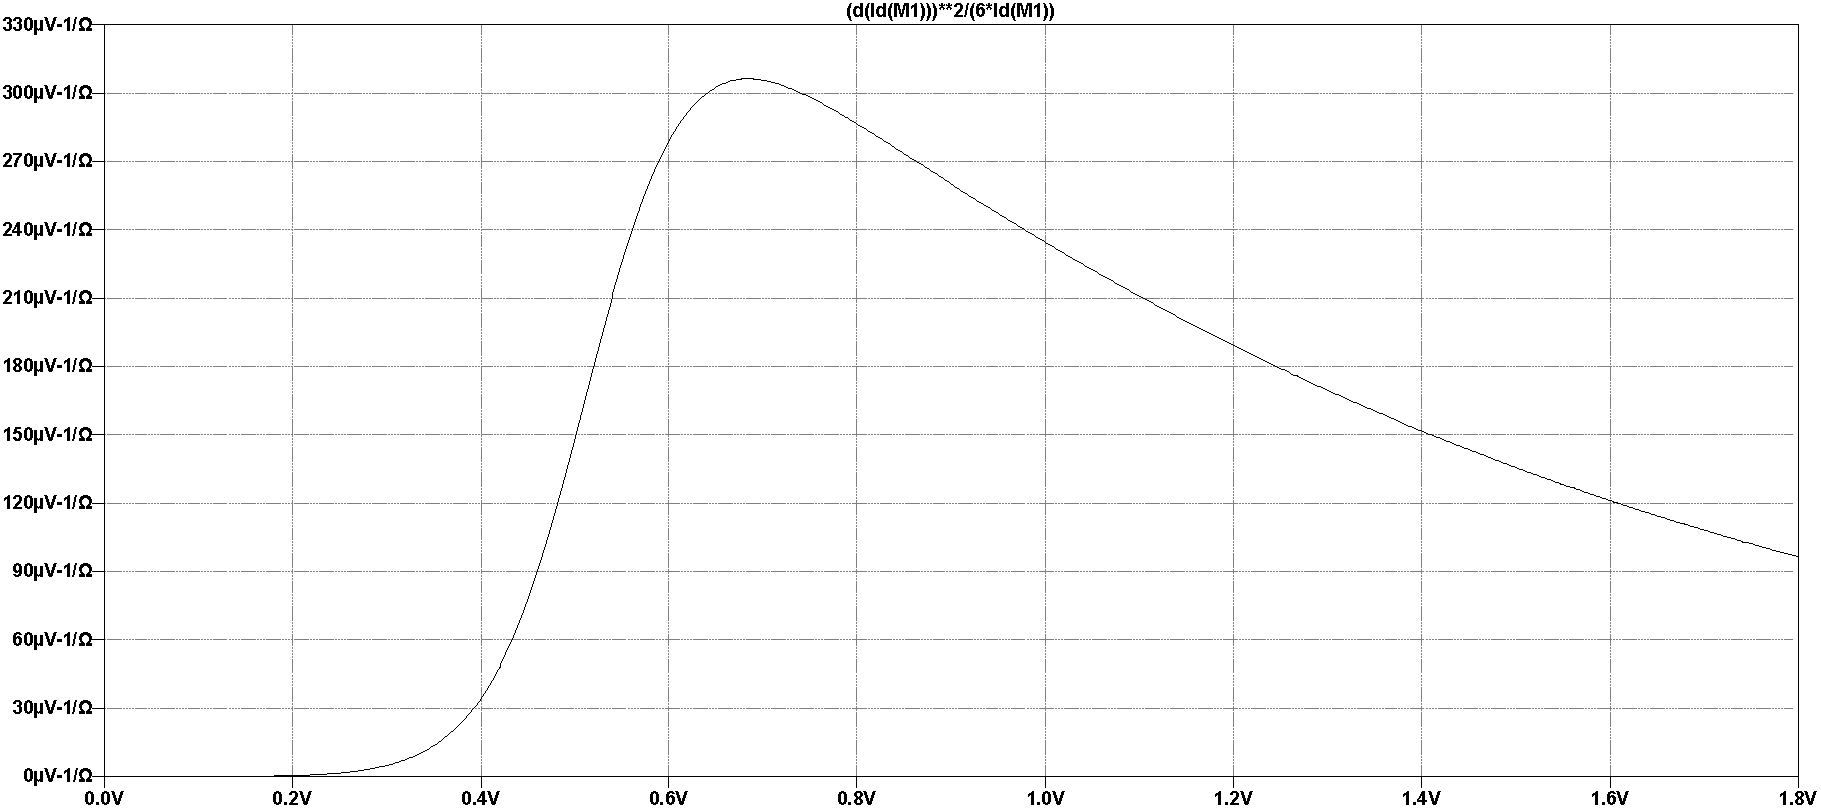
\includegraphics[width=.9\linewidth]{img/q3/b/nmos-ucox-vgs.pdf}
\caption{\label{fig:nmos-ucox-vgs}NMOS \(\mu\)\textsubscript{n}C\textsubscript{OX}-V\textsubscript{GS}}
\end{figure}
\item \(V_{THn} = 0.44V\)
\begin{figure}[H]
\centering
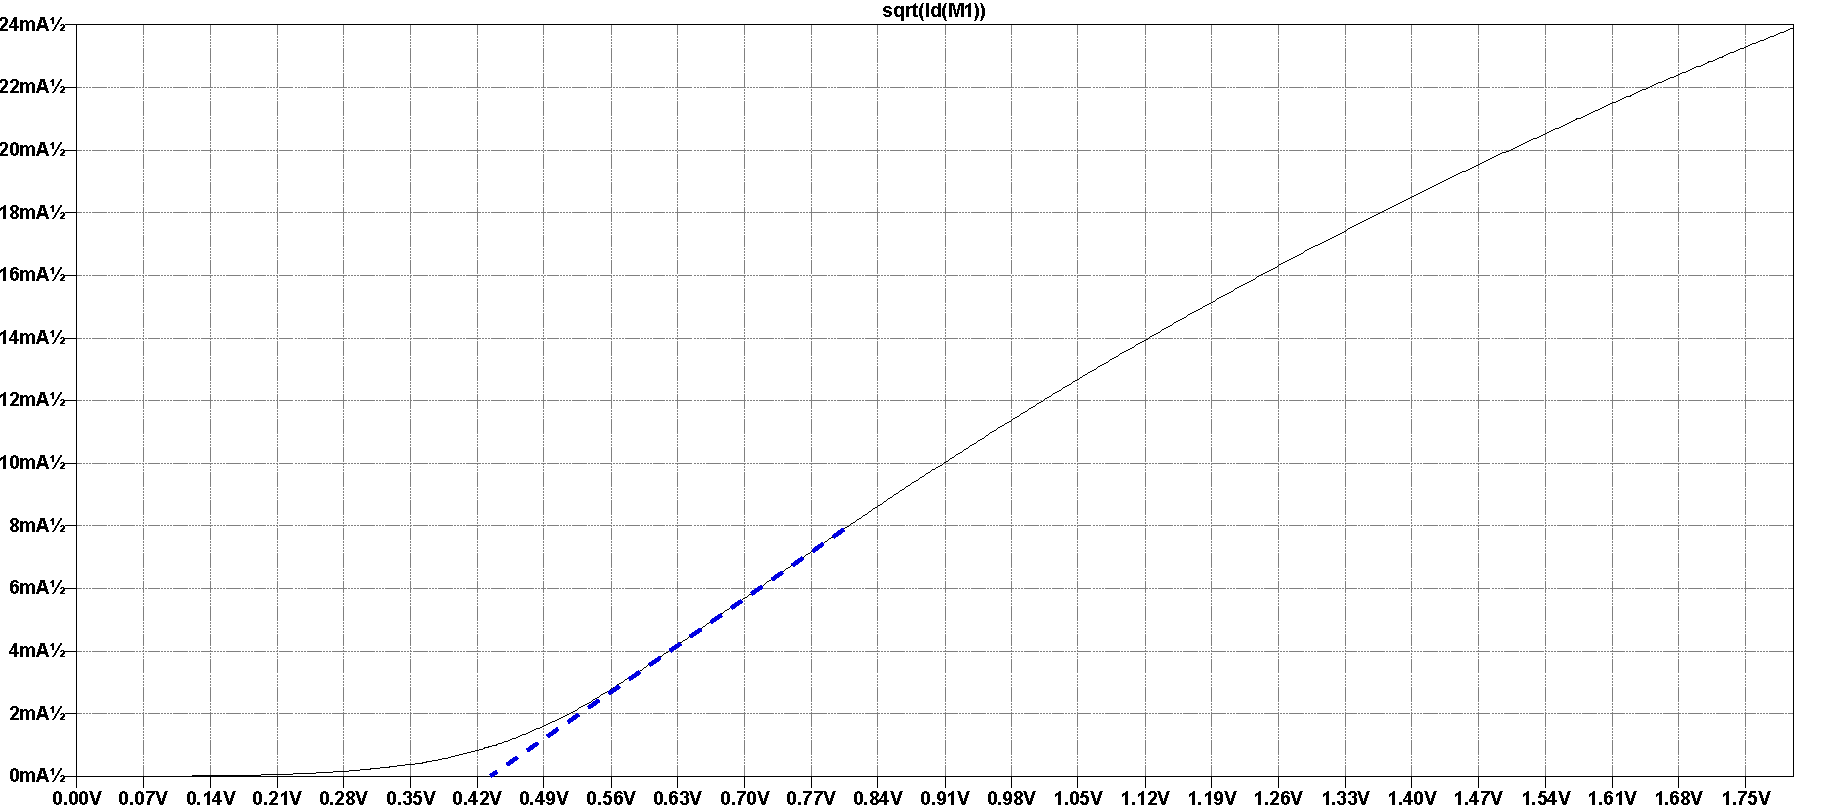
\includegraphics[width=.9\linewidth]{img/q3/b/nmos-sqrt-id-vgs.pdf}
\caption{\label{fig:nmos-sqrt-id-vgs}NMOS \(\sqrt{I_{D}}-V_{GS}\)}
\end{figure}
\end{enumerate}
\item PMOS
\begin{enumerate}
\item \(\mu_{p}C_{OX}\)
\item \(V_{THp}\)
\end{enumerate}
\end{enumerate}
\end{enumerate}

\section{Problem 4}
\label{sec:org783ffcc}
\section{Problem 5}
\label{sec:org2e0d414}
\section{Problem 6}
\label{sec:org4c8574b}
\section{Problem 7}
\label{sec:orga4a9cd0}
\end{document}
